\documentclass{beamer}
\usepackage{tikz}
\usetikzlibrary{arrows.meta, decorations.pathreplacing, calc}

% ------------------------------------------------------------------
% Theme colors & styles used below: blkline / blkfill / accentline /
% accentfill / lbl / flow. These are assumed to already exist in your
% master preamble (as in the stack-frame diagram you pasted) — delete
% this block if you're dropping the figure into that same file.
% ------------------------------------------------------------------
\definecolor{blkline}{HTML}{375775}
\definecolor{blkfill}{HTML}{EAF0F7}
\definecolor{accentline}{HTML}{B5651D}
\definecolor{accentfill}{HTML}{FBEEDD}
\tikzset{
  lbl/.style={text=black},
  flow/.style={-{Stealth[length=2.2mm]}, thick},
}

\begin{document}

\begin{frame}{LDR: Loading a Word from Memory (Little-Endian)}
\centering
\resizebox{0.92\textwidth}{!}{%
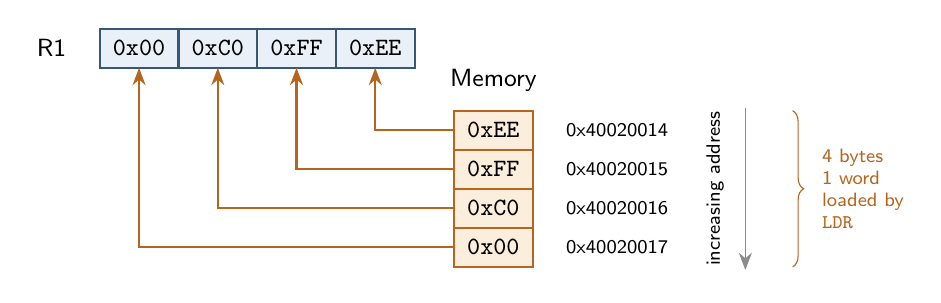
\begin{tikzpicture}[x=10mm, y=8mm]

\def\bw{1.0}    % width of one byte box
\def\rh{0.62}   % row height (matches the stack-frame diagram)

% --- Register R1: four contiguous byte boxes ---
\def\regx{0.7}
\def\regy{4.3}
\foreach \i/\val in {0/{0x00},1/{0xC0},2/{0xFF},3/{0xEE}}{
  \pgfmathsetmacro{\x}{\regx+\i*\bw}
  \draw[draw=blkline, fill=blkfill, thick]
      (\x,\regy) rectangle ({\x+\bw},{\regy-\rh});
  \node[font=\ttfamily\small] at ({\x+\bw/2},{\regy-\rh/2}) {\val};
}
\node[lbl, anchor=east, font=\sffamily\small] at ({\regx-0.3},{\regy-\rh/2}) {R1};

% --- Memory: four stacked byte boxes, addresses increasing downward ---
\def\memx{5.2}
\def\memy{3.0}
\foreach \i/\val/\addr in {%
    0/{0xEE}/{0x40020014},
    1/{0xFF}/{0x40020015},
    2/{0xC0}/{0x40020016},
    3/{0x00}/{0x40020017}}{
  \pgfmathsetmacro{\y}{\memy-\i*\rh}
  \draw[draw=accentline, fill=accentfill, thick]
      (\memx,\y) rectangle ({\memx+\bw},{\y-\rh});
  \node[font=\ttfamily\small] at ({\memx+\bw/2},{\y-\rh/2}) {\val};
  \node[lbl, anchor=west, font=\sffamily\scriptsize] at ({\memx+\bw+0.3},{\y-\rh/2}) {\addr};
}
\node[lbl, anchor=south, font=\sffamily\small] at ({\memx+\bw/2},{\memy+0.15}) {Memory};

% --- Arrows: bytes flow up from memory into the register (LDR) ---
\draw[flow, draw=accentline] (\memx,{\memy-0*\rh-\rh/2}) -| ({\regx+3*\bw+\bw/2},{\regy-\rh});
\draw[flow, draw=accentline] (\memx,{\memy-1*\rh-\rh/2}) -| ({\regx+2*\bw+\bw/2},{\regy-\rh});
\draw[flow, draw=accentline] (\memx,{\memy-2*\rh-\rh/2}) -| ({\regx+1*\bw+\bw/2},{\regy-\rh});
\draw[flow, draw=accentline] (\memx,{\memy-3*\rh-\rh/2}) -| ({\regx+0*\bw+\bw/2},{\regy-\rh});

% --- Address axis, to the right of the address column ---
\def\axisx{8.9}
\draw[-{Stealth[length=2.2mm]}, draw=black!45]
    ({\axisx},{\memy+0.05}) -- ({\axisx},{\memy-4*\rh-0.05});
\node[lbl, anchor=south, rotate=90, font=\sffamily\scriptsize]
    at ({\axisx-0.15},{\memy-2*\rh}) {increasing address};

% --- Brace naming the whole word ---
\draw[decorate, decoration={brace, amplitude=4pt}, draw=accentline]
    ({\axisx+0.6},{\memy}) -- ({\axisx+0.6},{\memy-4*\rh});
\node[lbl, anchor=west, align=left, font=\sffamily\scriptsize, text=accentline]
    at ({\axisx+0.85},{\memy-2*\rh}) {4 bytes\\1 word\\loaded by\\\texttt{LDR}};

\end{tikzpicture}%
}
\end{frame}

\end{document}
